\documentclass[]{article}
\usepackage[margin=1in]{geometry}
\usepackage[affil-it]{authblk}
\usepackage{gastex} % pictures on steroids
\usepackage{epsfig}
\usepackage{float}
\usepackage{graphicx}
\usepackage{caption}
\usepackage{subcaption}
\usepackage{amsmath}
%\usepackage{times}
%\usepackage{mathtime} 
\usepackage{pslatex} %regular times font/smaller courier font
\usepackage{amssymb}
\usepackage{alltt}
\usepackage{longtable}
\usepackage{multirow}
\usepackage{url}
\usepackage{mathrsfs} %for \mathscr{} 
\usepackage{multicol}
\usepackage{capt-of}
\usepackage[toc,page]{appendix}
\usepackage{booktabs}
\usepackage{listings}
\usepackage{color}
\usepackage{nomencl}
\usepackage{hyperref}
\usepackage[numbered]{mcode}




%opening
\title{3-D Printed Unmanned Aerial System Project}
\author{
Jessica Glass %\inst{1}
and Kristin Yvonne Rozier %\inst{1}
}
\affil{University of Cincinnati, Cincinnati, Ohio, USA \\
   \texttt{\{glassjp,rozierky\}@ucmail.uc.edu}
}
\date{\today}

\makenomenclature
\makeindex

\begin{document}

\maketitle


\begin{abstract}
The Laboratory for Temporal Logic (LTL) in Aerospace at the University of Cincinnati is designing a new, free-and-open-source, easy-manufacture (i.e. 3-D printable with COTS components) Unmanned Aerial System (UAS). The UAS will be designed specifically to maximally support System Health Management (SHM) capabilities needed to safely create intelligent, autonomous UAS.

\end{abstract}

\printnomenclature

\section{Background}
The LTL is proposing the idea of an open-source, easy manufactured, 3-D printable, COTS Unmanned Aerial System (UAS).  This UAS should be a platform which can be easily put together and used.  The idea is that this UAS will be used as an educational tool at various universities to further develop research areas on-board UAS  There is limited research and development in UAS due to the fact that the development of small, lightweight electronics has recently made small UAS flight possible.  When looking back 10-20 years ago, there were limited COTS components available which would have allowed for a small UAS to fly.  We are talking about a UAS which ranges in weight from 2-5 kilograms, keeping the payload less than or equal to about 1 kilogram.  Before the development of lithium ion batteries, it was mostly infeasible for battery powered flight on this small of a scale. There have been tons of advancements in the capabilities of 3-D printing which allows for rapid prototyping and easy manufacturing which has never before been possible.  It will be very important with our design to keep the operating reynolds number high enough, as done with previous military small UAS.  Achieving a higher reynold's number can only be done one of two ways: increase the stall velocity (perhaps making a bungee-cord launch) or increase the chord width (as seen done with Dragon Eye -- probably not ideal to a certain point, due to increased drag it would bring).   \\


\subsection{Related Work}

\begin{itemize}

\item {\bf Aerodynamic and Structural Design of a Small Nonplanar Wing UAV} \cite{Lan08} This paper discusses, in detail, the design process of a small, nonplanar wing UAS. The initial sizing of the aircraft was inspired by previously successful small UASs (mostly military aircraft).  By using data from the previous small UASs, the author has created a "design space" for all UASs which meet the same operational requirements.  The paper has presented the step-by-step design process for any small UAS, nonplanar or otherwise, by first beginning with an initial weight estimate.  After an initial estimate has been calculated, a design point may be chosen, and then the aircraft performance characteristics will be determined.  Once all of this has been determined, you are able to choose a propulsion system (propeller motor and battery combination) based on how much power is needed to fly the UAS. 

\item {\bf Aircraft Performance and Design - John D. Anderson} \cite{And99} Chapter 8 of this textbook focuses on the design of propeller driven aircraft.  John D. Anderson has divided the design of a propeller aircraft into 7 main "pivot points".  Because his design process assumes a gas powered piston engine, there are some aspects of the weight estimation (which assumes weight variation) that cannot be used for battery powered UAS purposes.  However, Anderson offers some very valuable insight as to how to configure the actual geometry of the aircraft based on the final weight estimation.  The seven pivot points also offer an iterative method as a way to finalize the design of the aircraft.

\end{itemize}

\subsubsection{Previously Successful Small UAS -With Visuals}

\begin{table}[H]
\begin{minipage}[b]{0.65\linewidth}
\begin{tabular}{*{1}{p{0.65\textwidth}}}
{\bf The Pointer} is a hand-launchable small UAS that was primarily used for military applications.  It has a wingspan of 108 inches, length of 72 inches, gross weight of 10 lbs, payload capacity of 2 lbs, and battery weight of 2.2 lbs. The flight duration capability ranged from 1 to 1.5 hours at an airspeed ranging from 22-50 mph.
\end{tabular}
\end{minipage}
\hfill
\begin{minipage}[b]{0.5\linewidth}
\begin{tabular}{*{1}{p{0.65\textwidth}}}
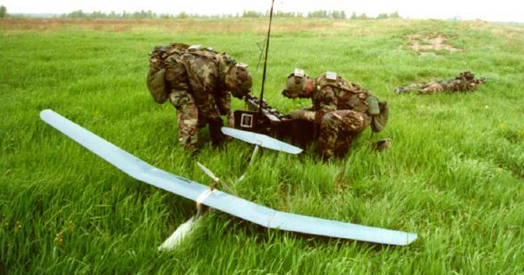
\includegraphics[height=8\baselineskip]{pointeruav}
\end{tabular}
\end{minipage}
\end{table}

\begin{table}[H]
\begin{minipage}[b]{0.65\linewidth}
\begin{tabular}{*{1}{p{0.65\textwidth}}}
{\bf The Raven} is a small hand-launchable UAS which was designed to replace the Pointer UAS.  It has a pusher-style electronic motor configuration.  The Raven has a wing span of 1.4 meters, length of 1.1 meter, a take-off weight of 1.9 kilograms, stall velocity of 8.68 m/s, and it has an endurance of about 1 hour and 20 minutes.
\end{tabular}
\end{minipage}
\hfill
\begin{minipage}[b]{0.5\linewidth}
\begin{tabular}{*{1}{p{0.65\textwidth}}}
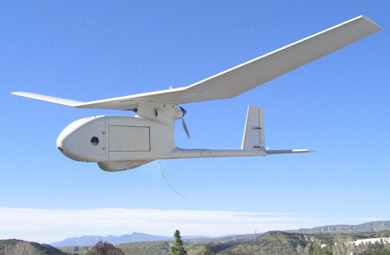
\includegraphics[height=8\baselineskip]{theraven}
\end{tabular}
\end{minipage}
\end{table}

\begin{table}[H]
\begin{minipage}[b]{0.65\linewidth}
\begin{tabular}{*{1}{p{0.65\textwidth}}}
{\bf The Puma} is another small, battery powered, hand-launchable UAS.  The puma has a wing span of 2.6 meters, length of 1.8 meters, a take off weight of 5.5 kilograms, stall velocity of 9.22 m/s, and an endurance of approximately 2 hours.  The Puma has a tractor-style electronic motor and a high-wing configuration.
\end{tabular}
\end{minipage}
\hfill
\begin{minipage}[b]{0.5\linewidth}
\begin{tabular}{*{1}{p{0.65\textwidth}}}
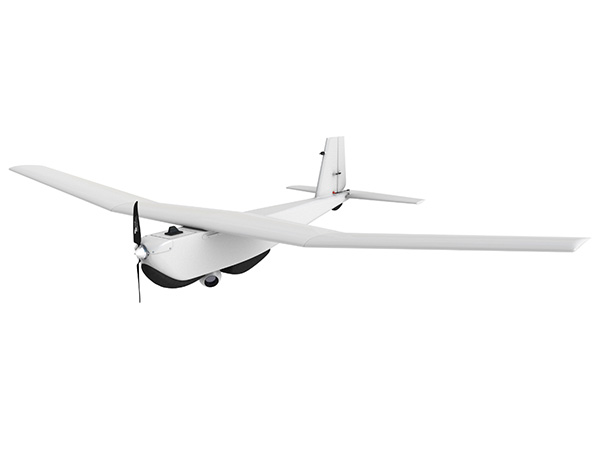
\includegraphics[height=8\baselineskip]{puma}
\end{tabular}
\end{minipage}
\end{table}

\begin{table}[H]
\begin{minipage}[b]{0.65\linewidth}
\begin{tabular}{*{1}{p{0.65\textwidth}}}
{\bf The Dragon Eye} is a small hand-launchable UAS designed to fit inside of a backpack.  It has a dual tractor-style motor configuration with a mid-wing.  The Dragon Eye has a wing span of 1.1 meters, a length of 0.9 meters, a take-off weight of 2.3 kilograms, stall velocity of 8.5 m/s, and an endurance of approximately 45 minutes.
\end{tabular}
\end{minipage}
\hfill
\begin{minipage}[b]{0.5\linewidth}
\begin{tabular}{*{1}{p{0.65\textwidth}}}
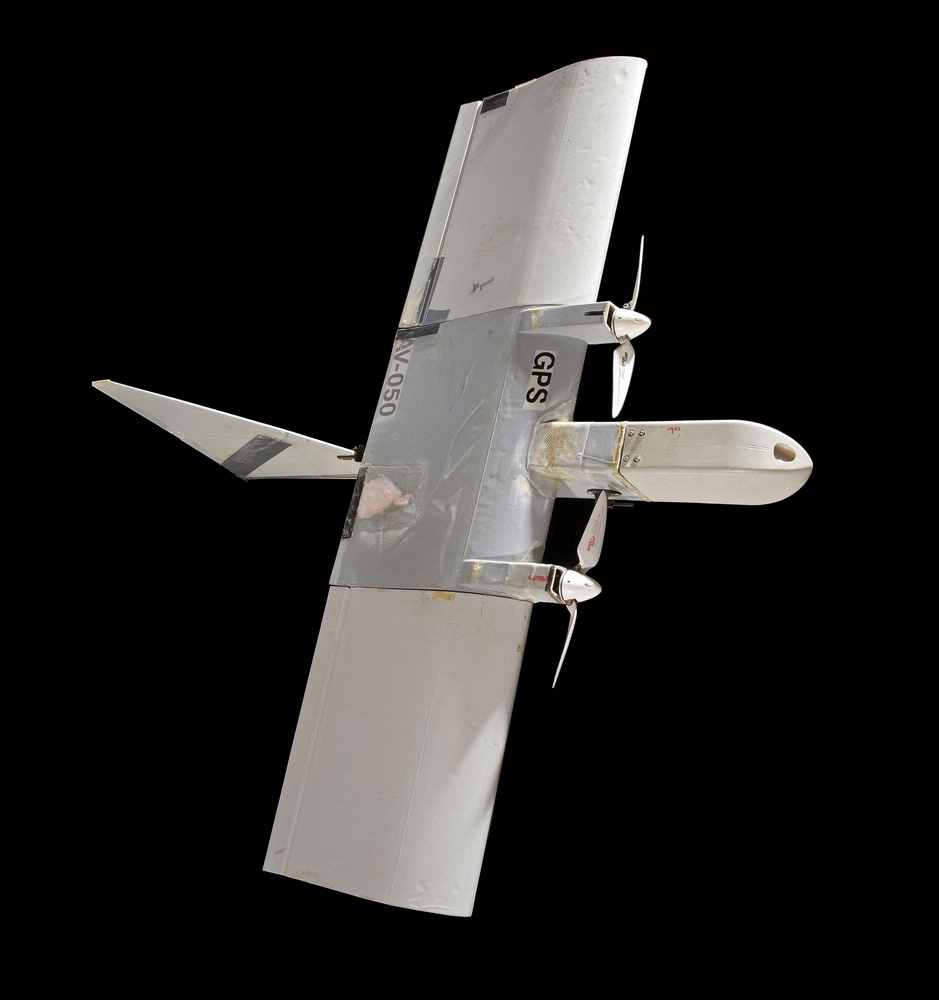
\includegraphics[height=8\baselineskip]{dragoneye}
\end{tabular}
\end{minipage}
\end{table}

\begin{table}[H]
\begin{minipage}[b]{0.65\linewidth}
\begin{tabular}{*{1}{p{0.65\textwidth}}}
{\bf The Desert Hawk} is a small, lightweight, portable UAS.  It has a wing span of 1.32 meters, length of 0.86 meters, take-off weight of 3.2 kilograms, stall velocity of 11.43 m/s, and an endurance of approximately 1 hour.  The Desert Hawk has a high-wing and tractor electric motor configuration.
\end{tabular}
\end{minipage}
\hfill
\begin{minipage}[b]{0.5\linewidth}
\begin{tabular}{*{1}{p{0.65\textwidth}}}
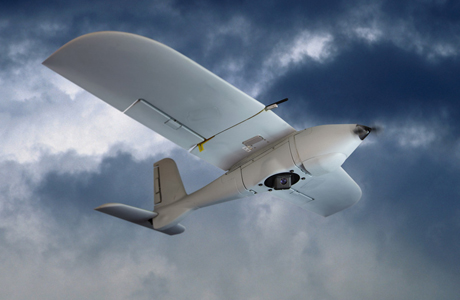
\includegraphics[height=8\baselineskip]{deserthawk}
\end{tabular}
\end{minipage}
\end{table}

\begin{table}[H]
\begin{minipage}[b]{0.65\linewidth}
\begin{tabular}{*{1}{p{0.65\textwidth}}}
{\bf The Orbiter} is a small UAS with a swept wing and pusher style motor configuration.  This aircraft has a span of 2.2 meters, length of 1 meter, take off weight of 5.5 kilograms, stall velocity of 12.75 m/s, and an endurance of 2.5 hours.  I would like to look into the benefits of the swept wing configuration and try to figure out why this was chosen -- perhaps to move C.O.G? Typically swept wings are used at high mach numbers.
\end{tabular}
\end{minipage}
\hfill
\begin{minipage}[b]{0.5\linewidth}
\begin{tabular}{*{1}{p{0.65\textwidth}}}
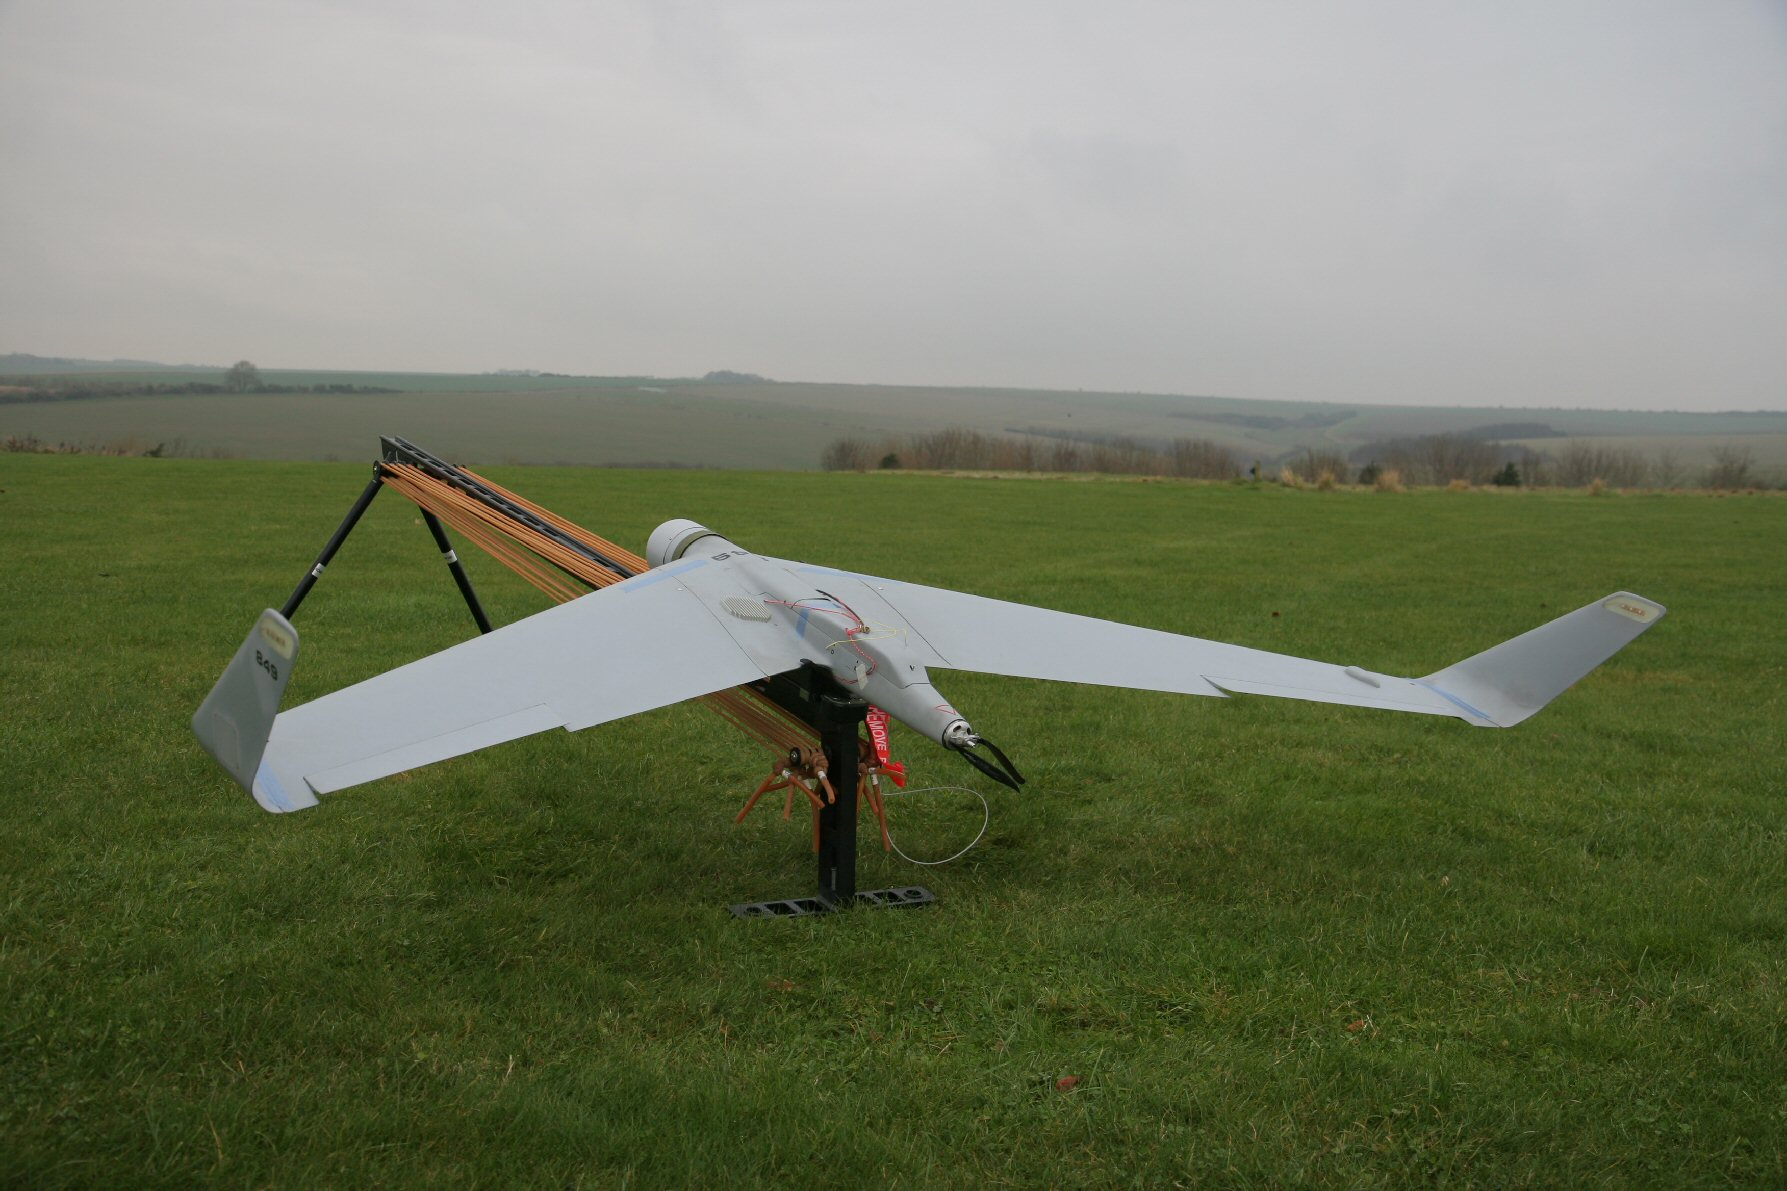
\includegraphics[height=8\baselineskip]{orbiter}
\end{tabular}
\end{minipage}
\end{table}



\begin{table}[H]
\begin{minipage}[b]{0.65\linewidth}
\begin{tabular}{*{1}{p{0.65\textwidth}}}
{\bf The Razor} is printed in nine parts that click together like DragonEye, with a similar one-piece fuselage with a removable hatch covering the cargo bay. Other independently-printed parts are: aileron, winglets, and mount for the small jet engine. \emph{(It is unclear what engine: we should find out.)} It is controlled by a Google Nexus 5 smartphone; UVA custom-designed an avionics app that controls the plane \emph{(let's find out if this is available)}. Razor has a four-foot wingspan, weighs 1.8 pounds empty and up to 6 pounds with sensors. The batteries take 2 hours to charge and are COTS. It can fly at 40 mph for up to 45 minutes with a max speed of 120 mph. The 3-D printing cost is \$800; phone, sensors, and other electronics cost \$1,700 for a total cost of \$2,500 per aircraft. The team found that 3-D printing lead to structural weaknesses in the aircraft, inspiring the flying-wing design.
\end{tabular}
\end{minipage}
\hfill
\begin{minipage}[b]{0.5\linewidth}
\begin{tabular}{*{1}{p{0.65\textwidth}}}
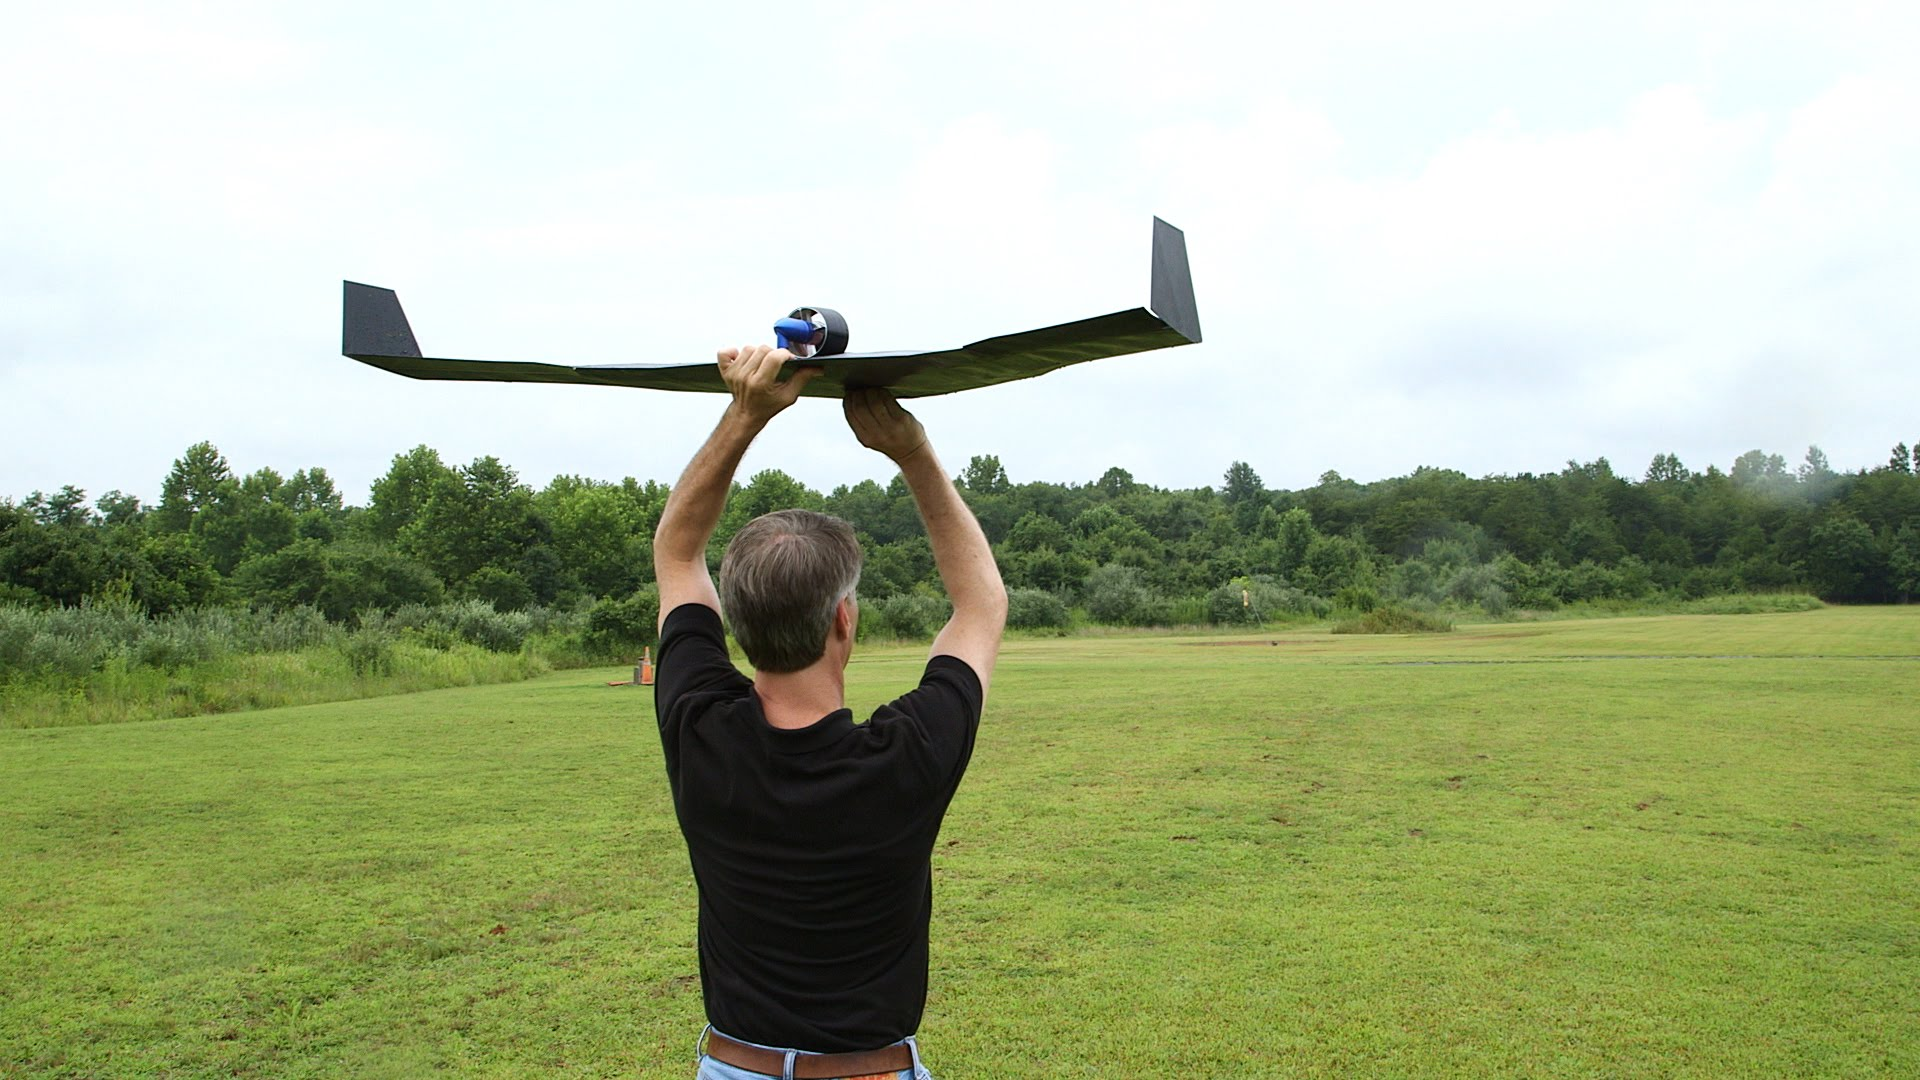
\includegraphics[height=8\baselineskip]{razor}
\end{tabular}
\end{minipage}
\end{table}


\subsection{Analysis}

The system health management (SHM) software and hardware were previously tested on NASA's retired military UAS, Dragon Eye and Swift.  These two UAS were not equipped to accommodate the SHM hardware and posed many challenges during the testing of RT-r2u2.  

\subsubsection{Challenges to Overcome}
\begin{itemize}

\item {\bf Challenges with DragonEye UAS} (Note: Seedling 2014 final deliverable technical report contains this too: \cite{RSI15}.)
  \begin{itemize}
    \item {\bf Overheating components} The Parallela Board overheats and shuts off due to lack of adequate cooling inside the DragonEye's only available compartment.
    \item {\bf Hard to maintain} The components are manufactured to fit exactly and glued into place. Re-connecting a loose wire requires many hours and possibly cutting into the UAS body.
    \item {\bf Short battery life} The battery lasts 1 hour maximum, but less with demanding sensors or operating at high speeds or after battery wear.
    \item {\bf Specialized components} The battery and other components are manufactured for the specific fuselage shape and difficult to replace when they wear out since they are not manufactured separately from the UAS.
  \end{itemize}

\item {\bf Challenges with Swift UAS}
  \begin{itemize}
    \item {\bf Requires runway for take-off and landing} The need to schedule a full-sized runway where passenger planes can take off limits possibilities for flight testing.
    \item {\bf Hard to ship to different flight test locations} The 13-foot wingspan binds this UAS to one airport.
  \end{itemize}

\end{itemize}


\subsubsection{Our Requirements}
This led us to develop the following set of requirements for the design of our UAS:

\begin{itemize}
  \item Easily re-configurable to accomodate different sensor suites and adequate internal cooling fans
  \item Long battery life to enable distance missions where autonomy is required
  \item Small size that enables flight testing at a variety of locations without requiring a full-sized runway
  \item Easily de-composable for easy transportation to flight testing location
  \item 3D printable parts
\end{itemize}





\section{Design Iteration Method}
This section will go into detail explaining the iteration method of design, referencing both the thesis paper and the aircraft performance text book, will also show the breakdown of our initial weight estimate based on the payload of the iron bird, maybe illustrate MATLAB code written to reproduce thesis paper's design space

\subsection{Related Work}

\subsubsection{"The Seven Intellectual Pivot Points for Conceptual Design"}*cite aircraft performance and design*

\begin{itemize}

\item 1. {\bf Requirements} This is where you establish the set of requirements the aircraft must meet.  Some typical requirement aspects include: range, takeoff distance, stalling velocity, endurance, maximum velocity, rate of climb, maximum load factor, cost, reliability and maintainability, and maximum size.

\item 2. {\bf Weight of the Airplane - First Estimate} Getting an initial estimate of the airplane's weight is important for determining the performance parameters.

\item 3. {\bf Critical Performance Parameters}  This is where we will choose our airfoil and calculate our initial performance parameters.  Things such as clmax, L/D, W/S, T/W, etc....

\item 4. {\bf Configuration Layout} Here we will determine more specifics about the design of our aircraft.  For example: tractor vs pusher motor configuration, high wing vs mid wing configuration, taper ratio (if any at all, can be used to decrease structural weight, increase AR), and weight distrubution.

\item 5. {\bf Better Weight Estimate} This is where, based on the configuration determined above, we can come to a better weight estimate based on the material we will be using.  

\item 6. {\bf Performance Analysis} Are we meeting or exceeding our requirements?  If not, iterate steps until we converge on a solution.

\item 7. {\bf Optimization} Is this the best design?

\end{itemize}

\subsubsection{Constraint Equations} 

The design of a propeller driven aircraft is constrained by the following equations: \\

Max Load/Turn:
\begin{equation}
\frac{HP}{W}= \frac{1}{550\eta_{p}}[\frac{1}{2}\rho V^{3} C_{D_{O}} (\frac{S}{W}) + 2K \frac{n^2}{\rho V} (\frac{W}{S})]
\end{equation}

Endurance:
\begin{equation}
\frac{HP}{W}=\frac{4}{550\eta_{p}} C_{D_{O}}^{1/4} (\frac{K}{3})^{3/4} (\frac{2}{\rho} \frac{W}{S})^{1/2}
\end{equation}

Cruise:
\begin{equation}
\frac{HP}{W}=\frac{2}{550\eta_{p}} C_{D_{O}}^{1/4} K^{3/4} (\frac{2}{\rho} \frac{W}{S})^{1/2}
\end{equation}

Takeoff Distance:
\begin{equation}
\frac{HP}{W}=\frac{2.44}{550\eta_{p}} \frac{1}{gd_{to}}(\frac{1}{\rho_{SL} C_{L_{max}}} \frac{W}{S})^{3/2}
\end{equation}

Stall Condition
\begin{equation}
\frac{W}{S}= \frac{\rho}{2} C_{L{max}} V_{SO}^2
\end{equation}

\noindent These equations allow us to create our design space in terms of $\frac{HP}{W}$ (horsepower to weight ratio) and $\frac{W}{S}$ (Wing loading)
%
\nomenclature{$\frac{HP}{W}$}{Horse Power to Weight Ratio}%








\subsection{Analysis}
This MATLAB code recreates the design space discussed from related work documents and allows user inputs in order to test values and get basic flight performance parameters in return

\lstinputlisting{UAS.m} 

\begin{figure}[H]
\centering
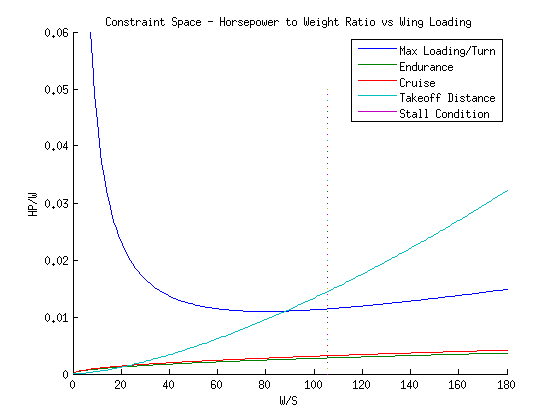
\includegraphics[scale=.75]{matlabdesignspace}
\caption{Design Constraint Space}
\end{figure}

\begin{figure}[H]
\centering
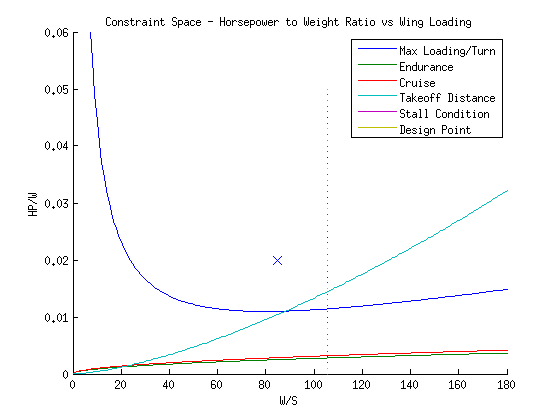
\includegraphics[scale=.75]{designspacewithpoint}
\caption{Design Constraint Space with User Input Design Point}
\end{figure}

\begin{figure}[H]
\centering
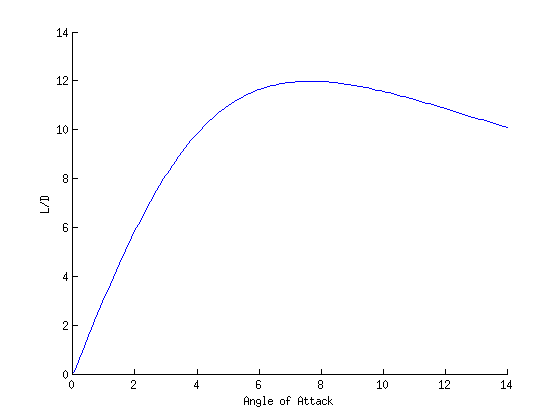
\includegraphics[scale=.75]{ldaoaexample}
\caption{Output Graph - L/D ratio vs AOA}
\end{figure}


\section{Aerodynamics}
This section will be mostly visual, containing all 2D airfoil analysis performed.  It will also reference (at least) 2 aerodynamics textbooks regarding 2D flow analysis.  

\subsection{Related Work}
The aerodynamic body is better described by the force and moment coefficients, rather than the actual forces and moments.  $C_{L}$, $C_{D}$, and $C_{M}$ can be described by the following equations:

\begin{equation}
C_{L} = \frac{L}{q_{\infty} S}
\end{equation}

\begin{equation}
C_{D} = \frac{D}{q_{\infty} S}
\end{equation}

\begin{equation}
C_{M} = \frac{M}{q_{\infty} Sc}
\end{equation}

where $q_{\infty}$ is the dynamic pressure, defined by

\begin{equation}
q_{\infty} = \frac{1}{2} \rho V_{\infty}^{2}
\end{equation}

and $c$ is the chord length of an airfoil.  We can also define the following parameters: \\

Reynolds Number:

\begin{equation}
Re = \frac{\rho_{\infty} V_{\infty} c}{\mu_{\infty}}
\end{equation}

Mach Number:

\begin{equation}
M_{\infty} = \frac{V_{\infty}}{a_{\infty}}
\end{equation}

From these equations, we know that for any given body shape, 

\begin{equation}
C_{L} = f_{1} (\alpha, Re, M_{\infty})
\end{equation}

\begin{equation}
C_{D} = f_{2} (\alpha, Re, M_{\infty})
\end{equation}

\begin{equation}
C_{M} = f_{3} (\alpha, Re, M_{\infty})
\end{equation}

For a two-dimensional airfoil, the lift, moment, and drag coefficients are written in lowercase letters and subscripts, $c_{l}$, $c_{d}$, and $c_{m}$.  These coefficients vary with both angle of attack and Reynolds number, which is depicted for several different airfoils in the subsequent section.  The lift curve (lift versus angle of attack) is one analysis of great importance.  The variance of $c_{l}$ over a range of angles of attack is typically linear, and the slope of this line is defined as the lift slope.  The lift slope is designated in most literature as $a_{0}$.  The theoretical value of $a_{0}$ for thin airfoils is $2\pi$ per radian or 0.11 per degree.  This can typically be used as a good approximation for most conventional airfoils.  Also on this lift curve, there will be a finite value of $\alpha$ for which the $c_{l} =0$ .  This angle of attack can be defined by $\alpha_{L=0}$.  Any positively cambered airfoil will have a negative $\alpha_{L=0}$, a symmetric airfoil will have $\alpha_{L=0} = 0$, and negatively cambered airfoils will have a positive $\alpha_{L=0}$, however negative cambered airfoils are not of practical interest.  On the other hand, when reaching the high end of the angle of attack spectrum, every airfoil will have a $c_{l_{max}}$ value.  The lift curve will peak at $c_{l_{max}}$, and then drop as angle of attack increases.  This is also known as the stall condition.  When the airfoil reaches the stall angle of attack ($c_{l_{max}}$), it causes flow separation on the top of the airfoil which will cause changes in the pressure differential which allowed this airfoil to fly in the first place.  The value of $c_{l_{max}}$ will vary with Reynolds number.  Typically, as Reynolds number increases, so does the value of $c_{l_{max}}$.

\subsection{Analysis}

Several airfoils have been selected (from \url{http://m-selig.ae.illinois.edu/ads/coord_database.html}) and analyzed using xflr5. Below are screenshots of the batch analysis performed on each airfoil. \\

\begin{figure}[H]
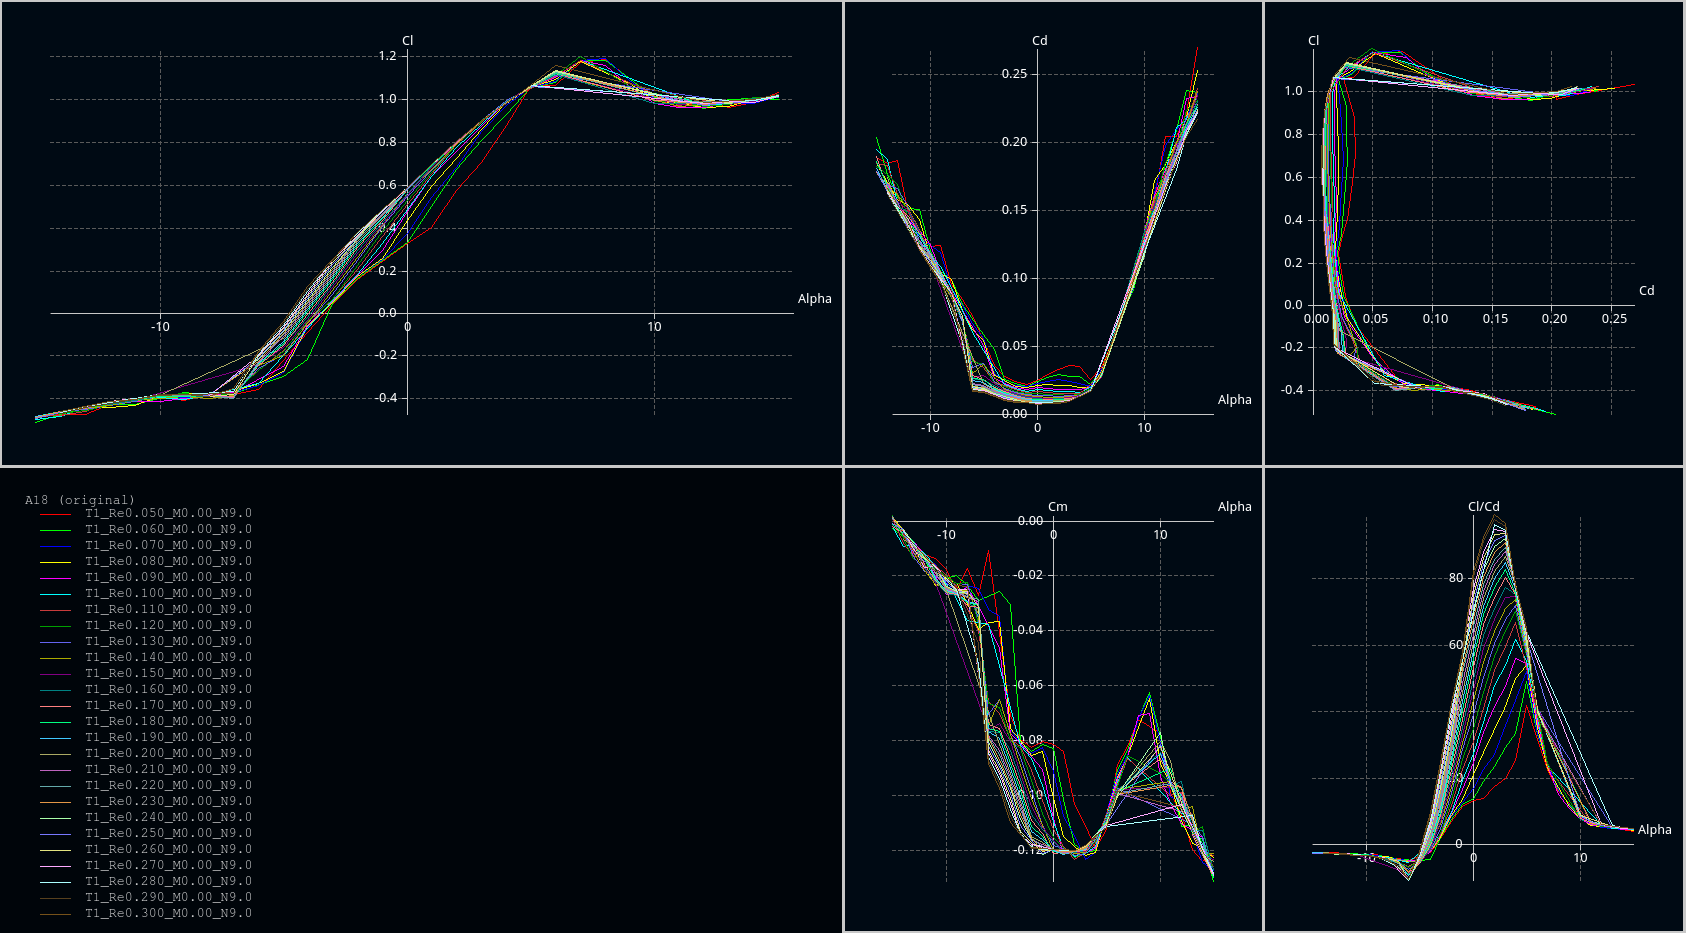
\includegraphics[scale=0.4]{a18_batch}
\caption{A-18 Airfoil Batch Analysis}
\end{figure}

\begin{figure}[H]
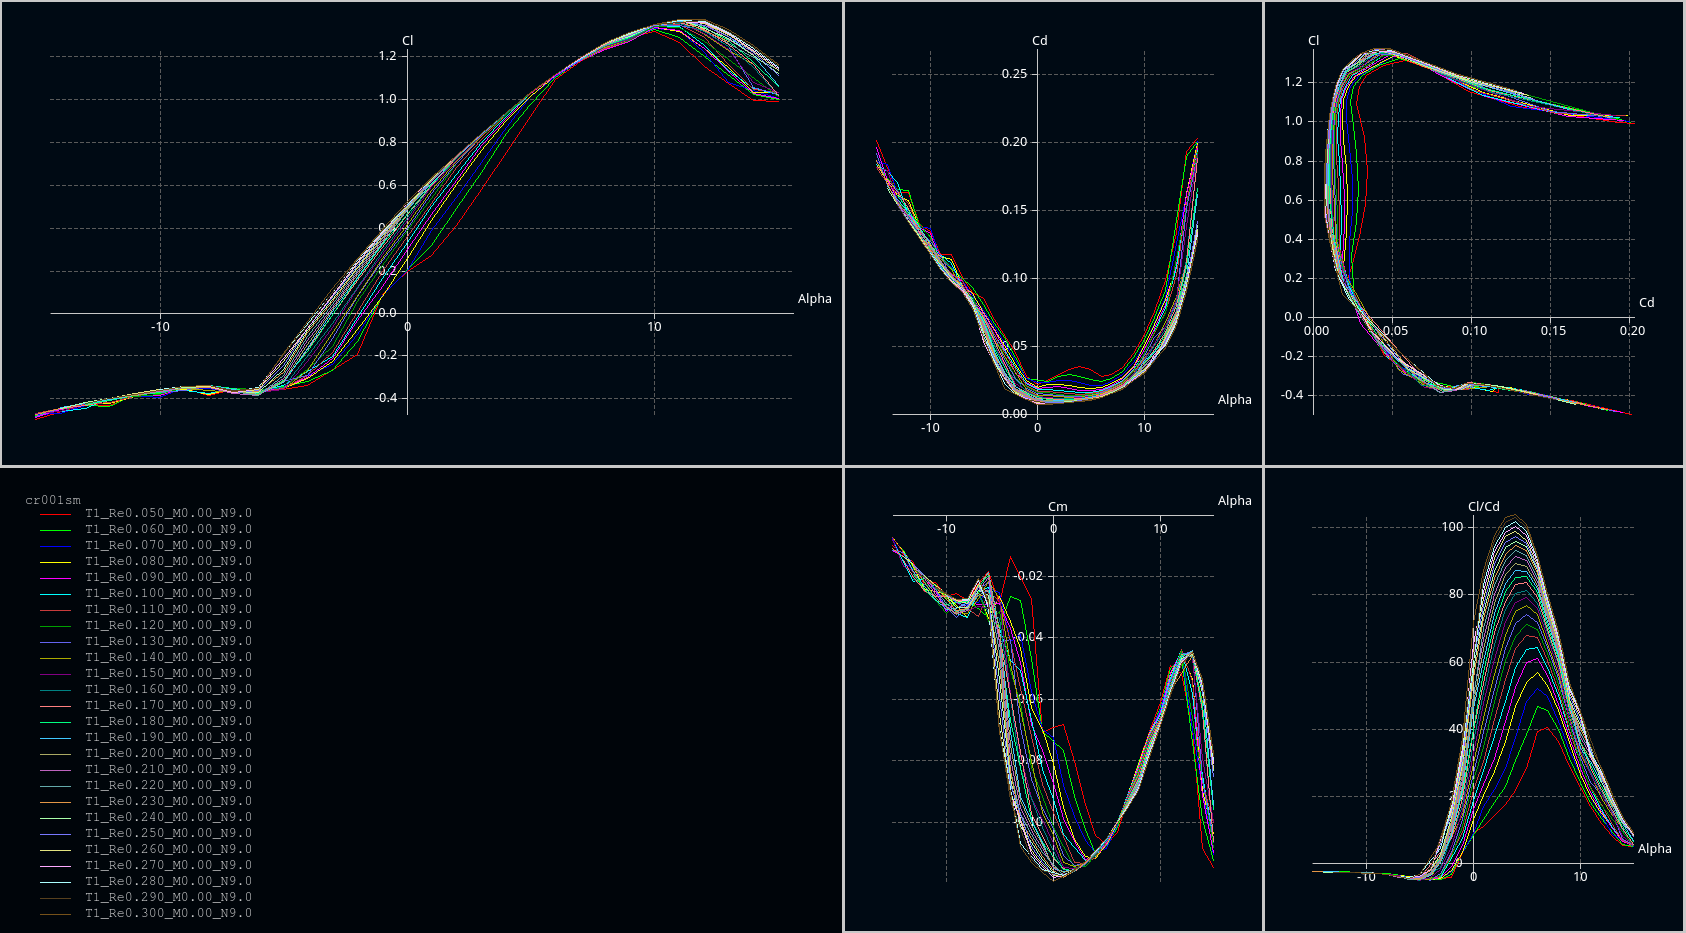
\includegraphics[scale=0.4]{cr001sm_batch}
\caption{CR001 Smooth Airfoil Batch Analysis}
\end{figure}

\begin{figure}[H]
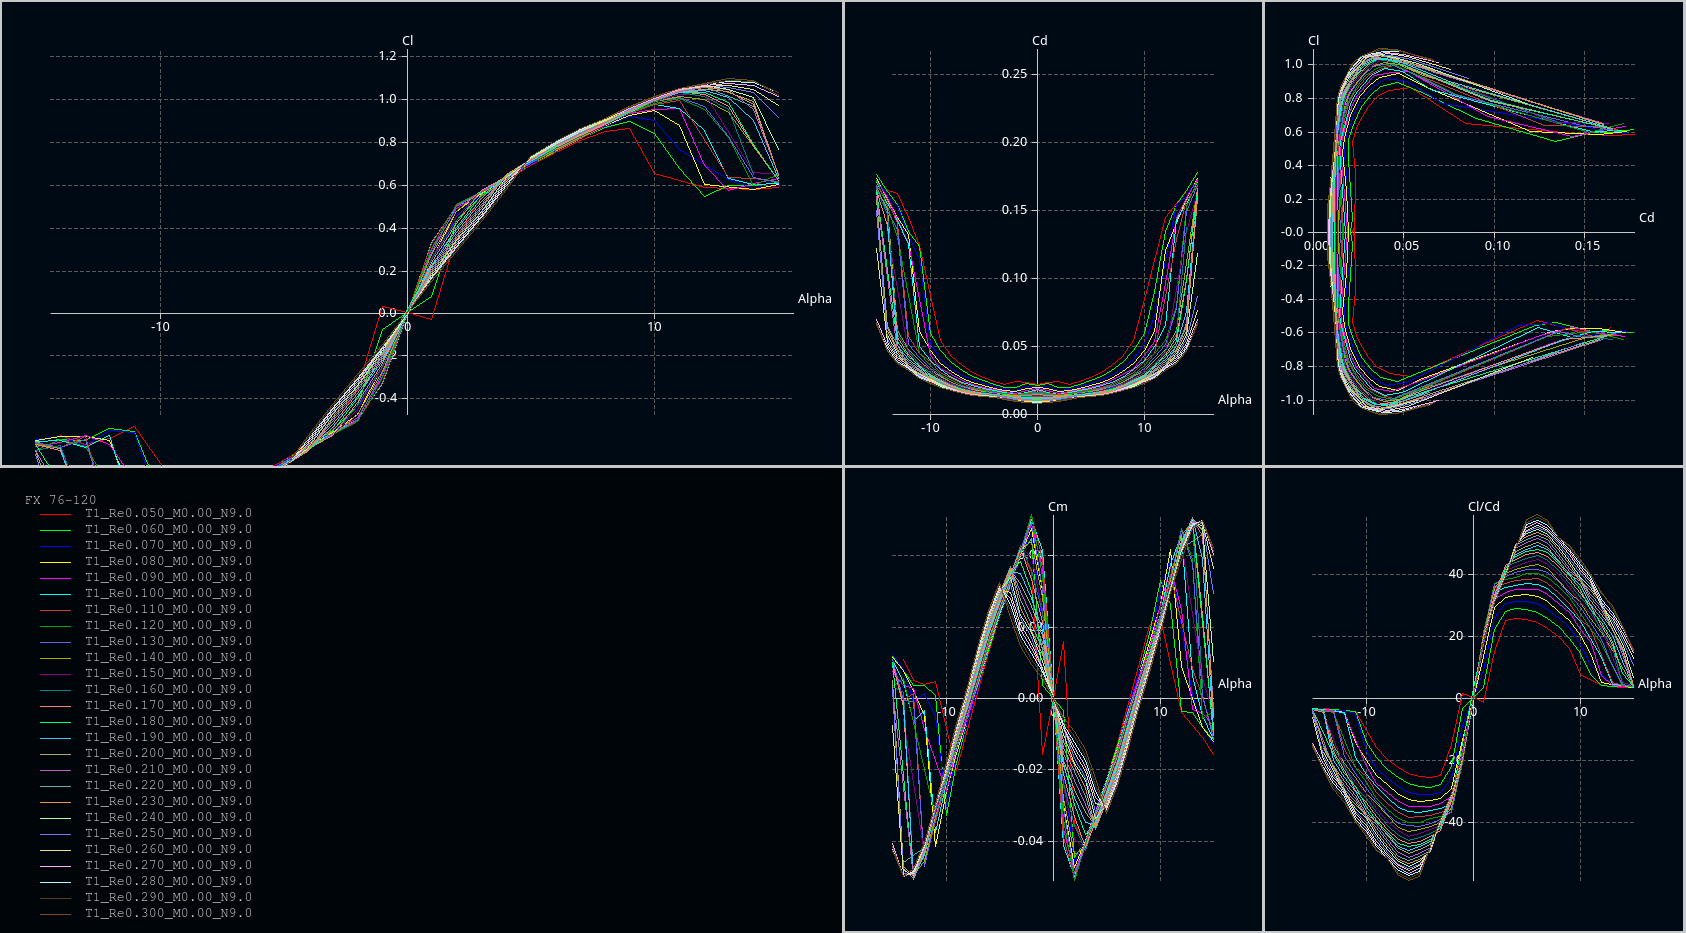
\includegraphics[scale=0.4]{fx76-120_batch}
\caption{FX76-120 Airfoil Batch Analysis}
\end{figure}

\begin{figure}[H]
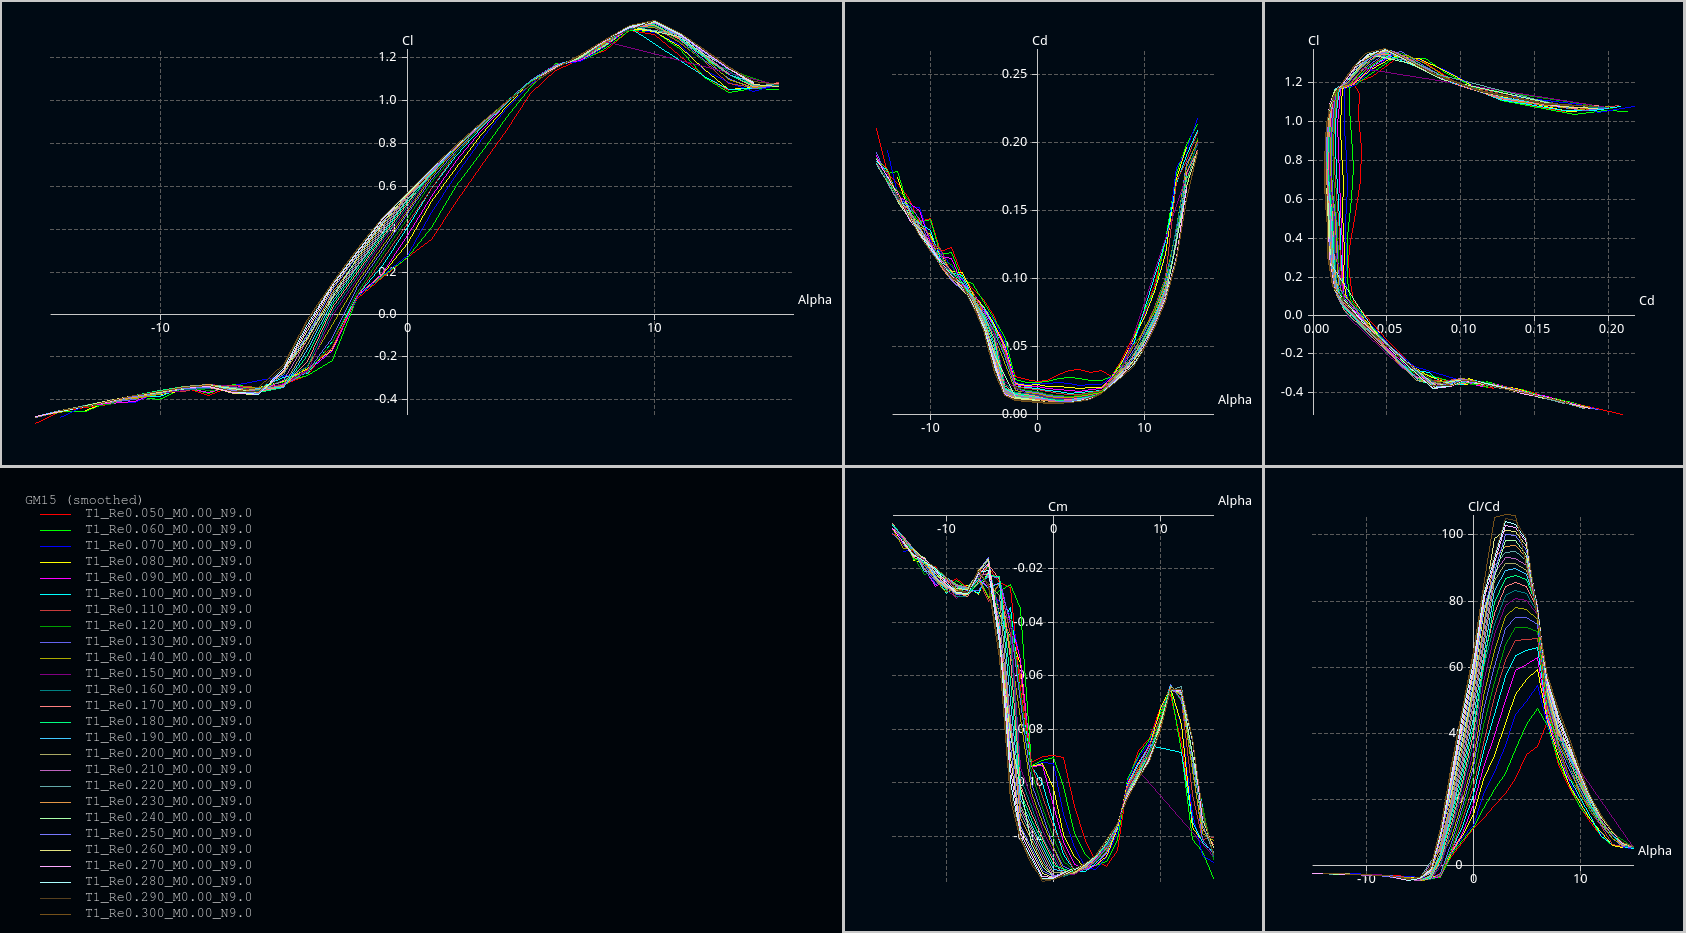
\includegraphics[scale=0.4]{gm15sm_batch}
\caption{GM15 Smooth Airfoil Batch Analysis}
\end{figure}

\begin{figure}[H]
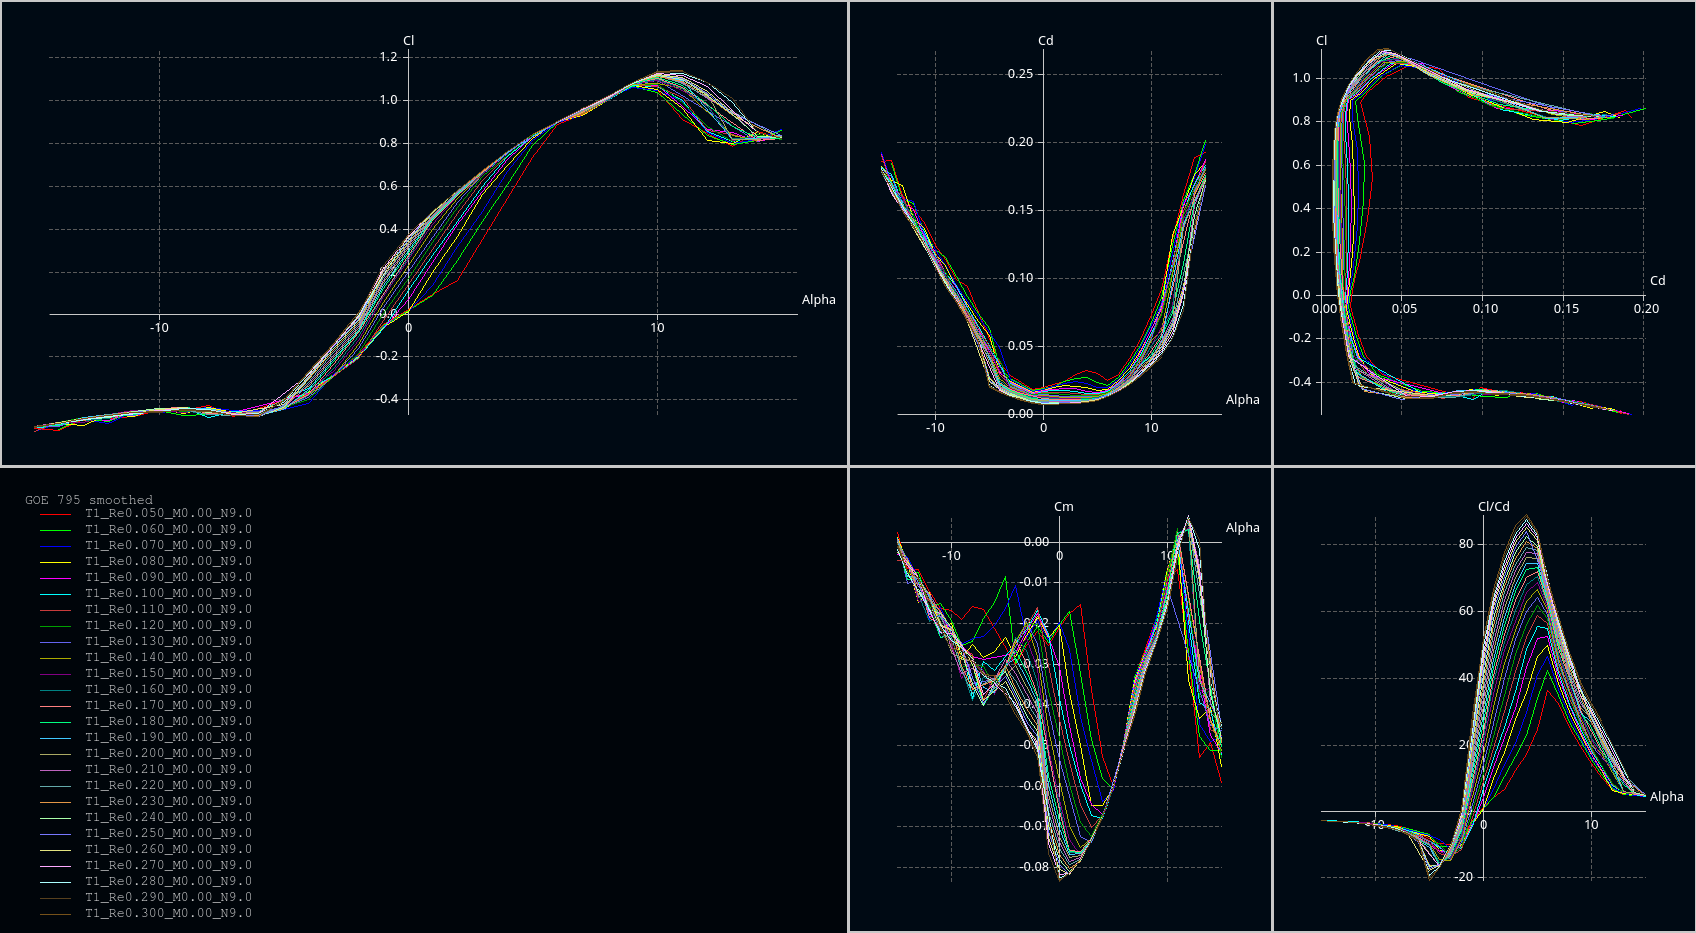
\includegraphics[scale=0.4]{goe795sm_batch}
\caption{GOE795 Smooth Airfoil Batch Analysis}
\end{figure}

\begin{figure}[H]
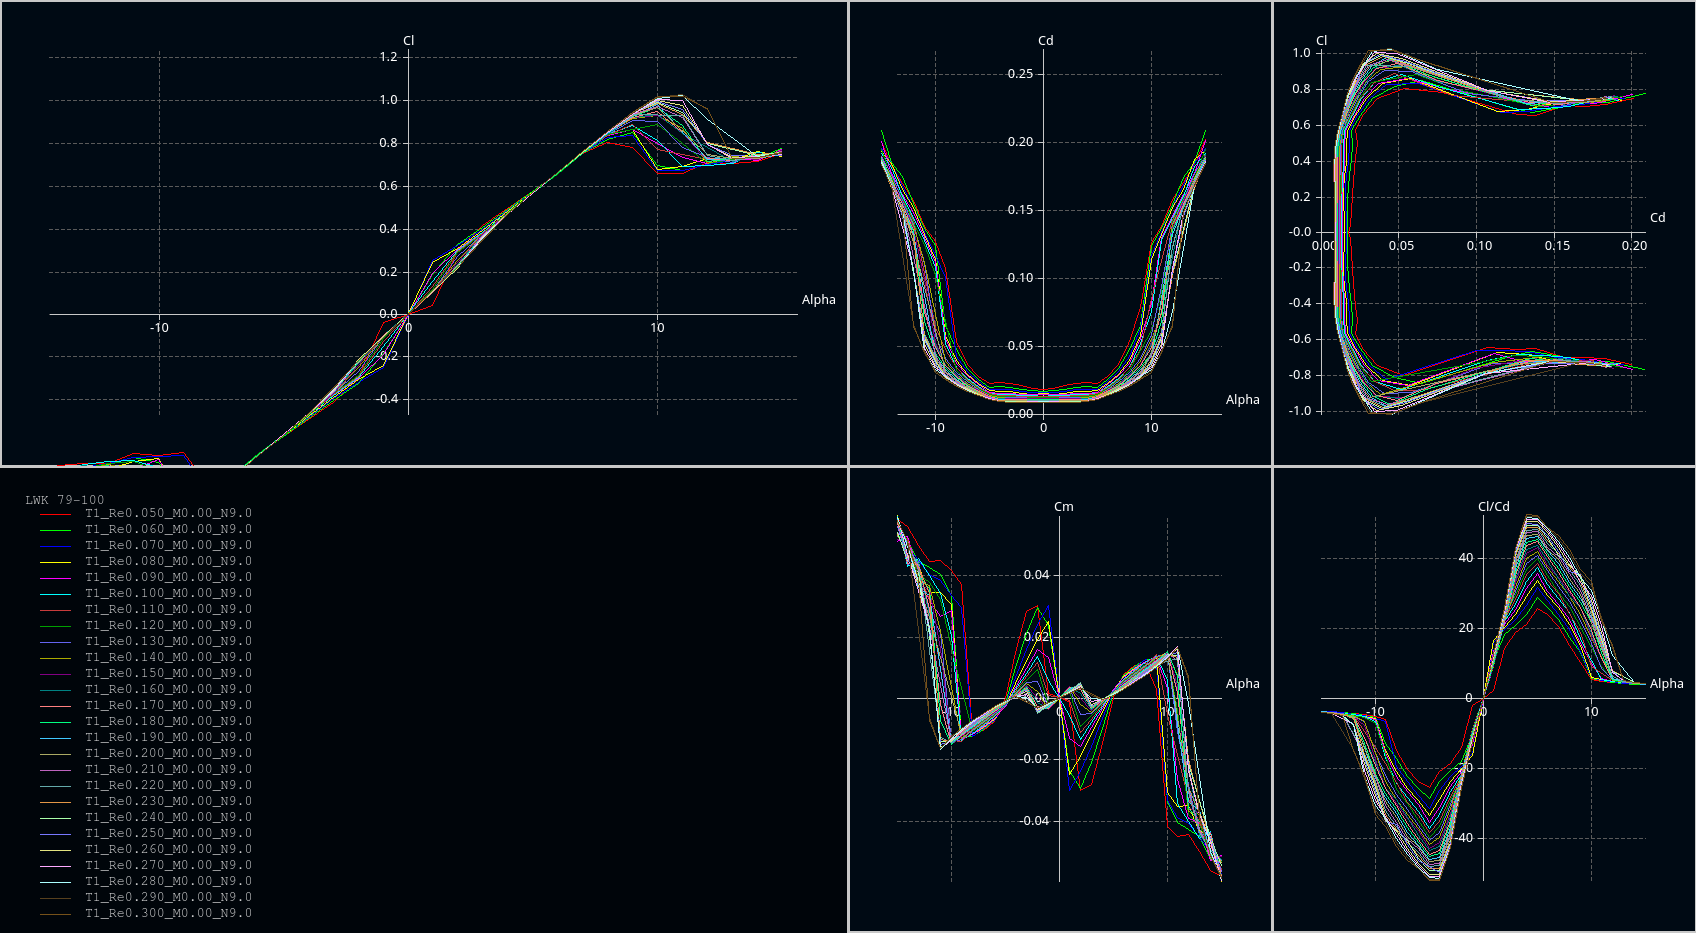
\includegraphics[scale=0.4]{lwk79-100_batch}
\caption{LWK79-100 Airfoil Batch Analysis}
\end{figure}

\begin{figure}[H]
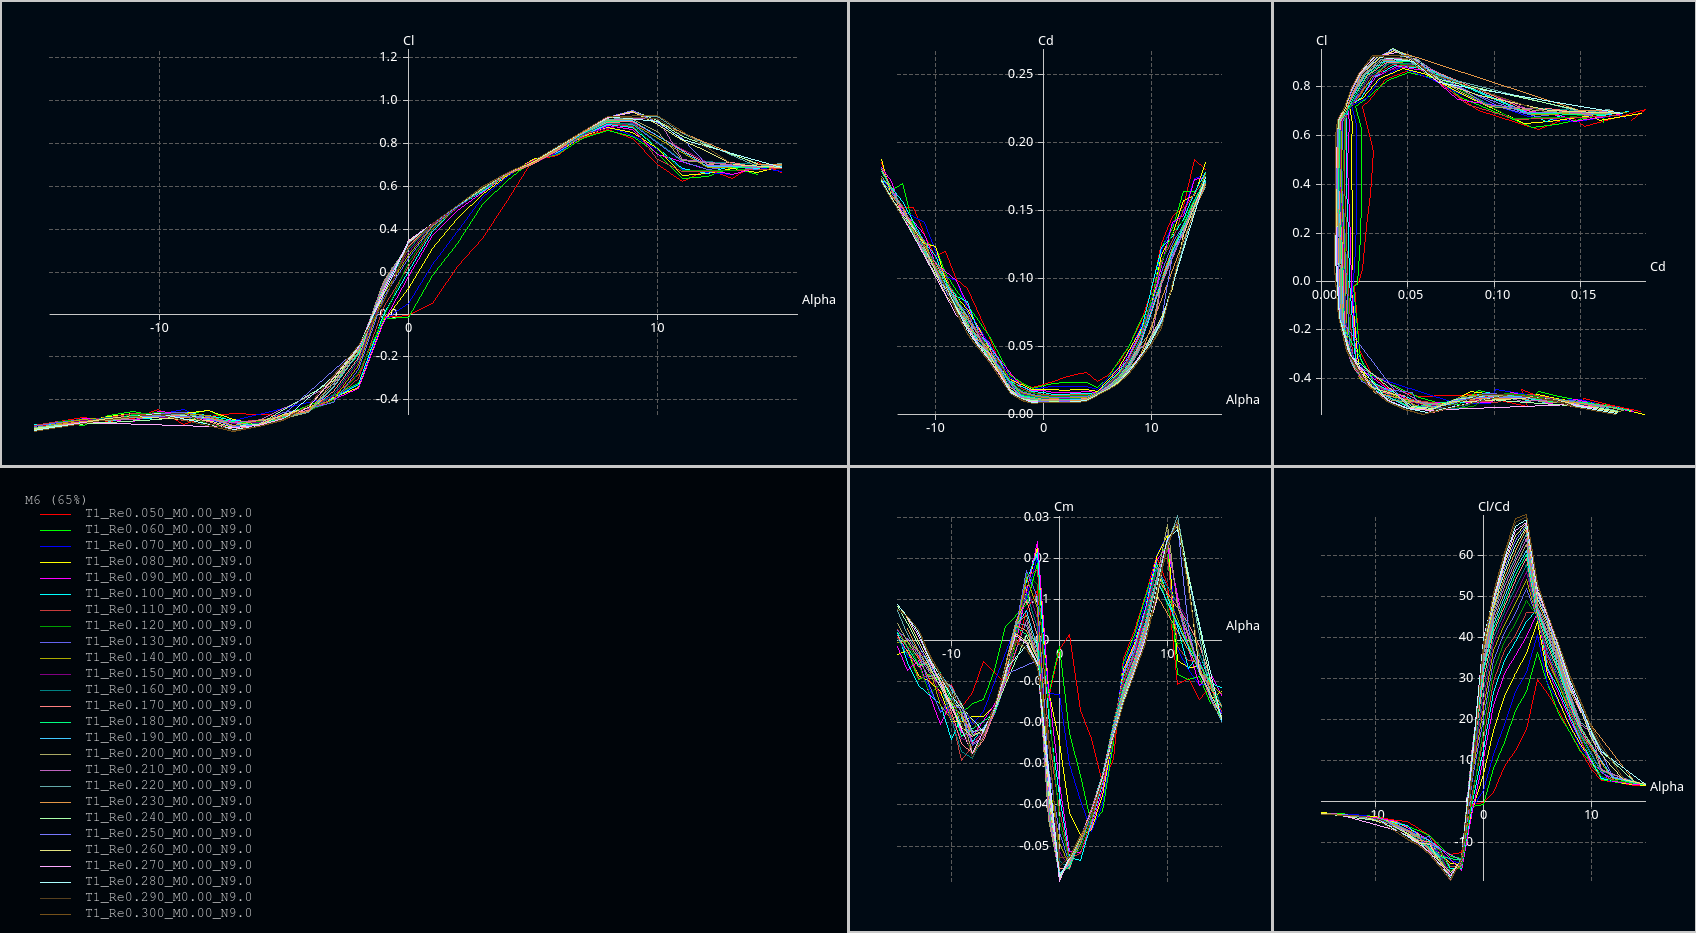
\includegraphics[scale=0.4]{m665_batch}
\caption{M665 Airfoil Batch Analysis}
\end{figure}

\begin{figure}[H]
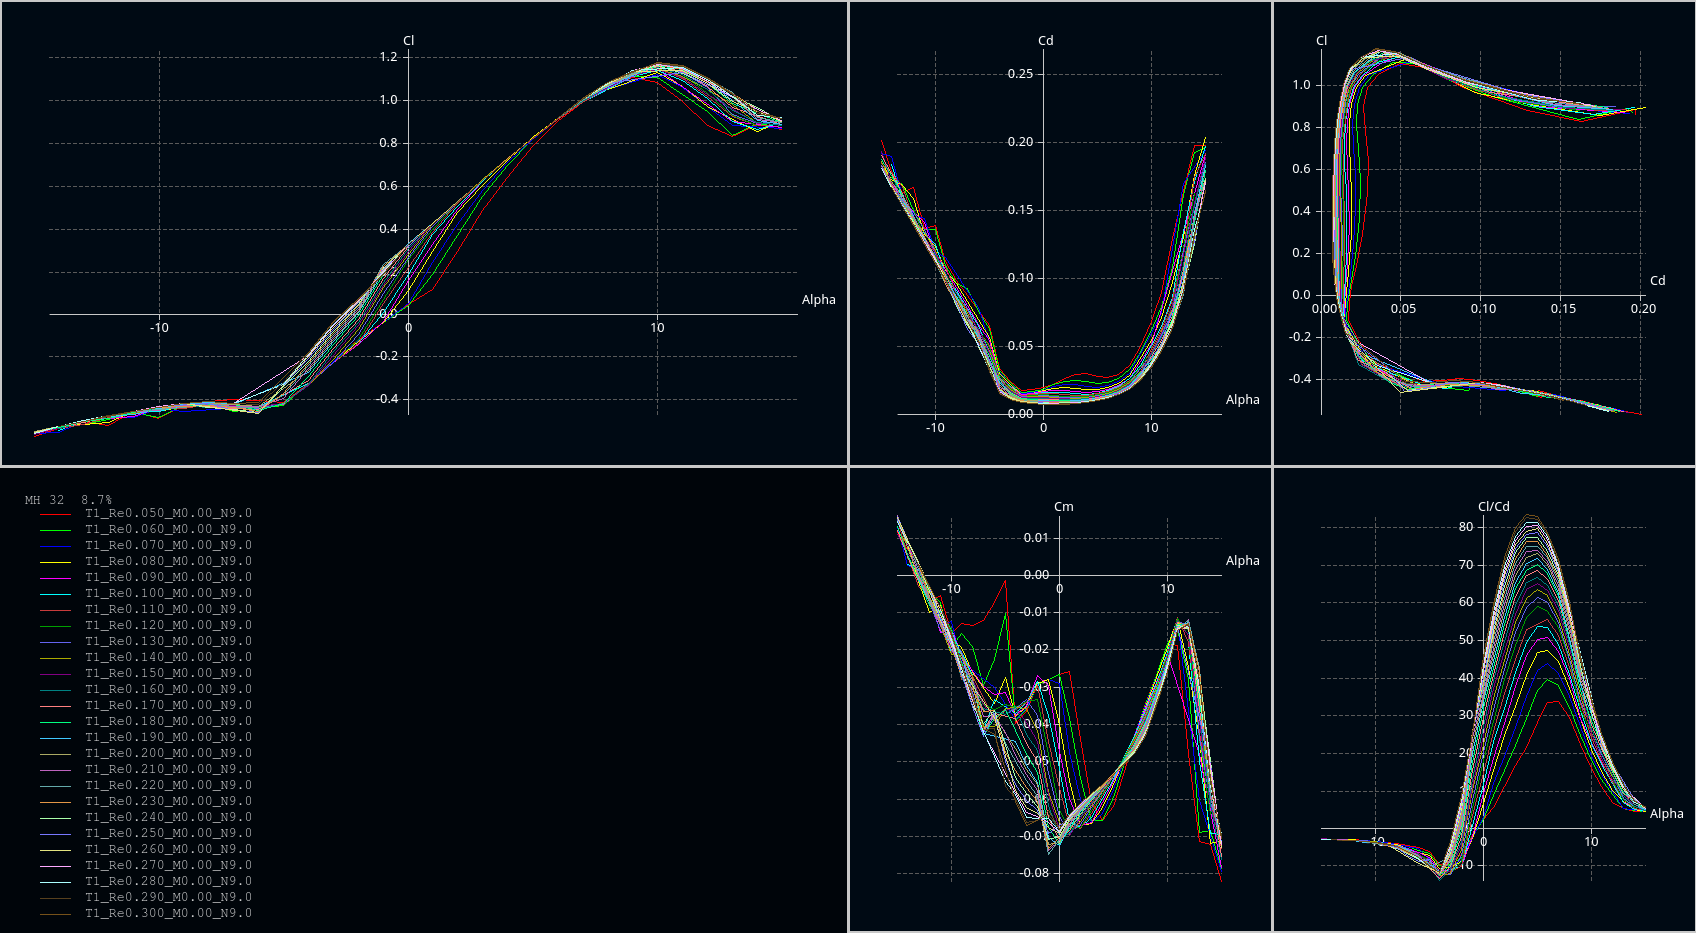
\includegraphics[scale=0.4]{mh32_batch}
\caption{MH32 Airfoil Batch Analysis}
\end{figure}

\begin{figure}[H]
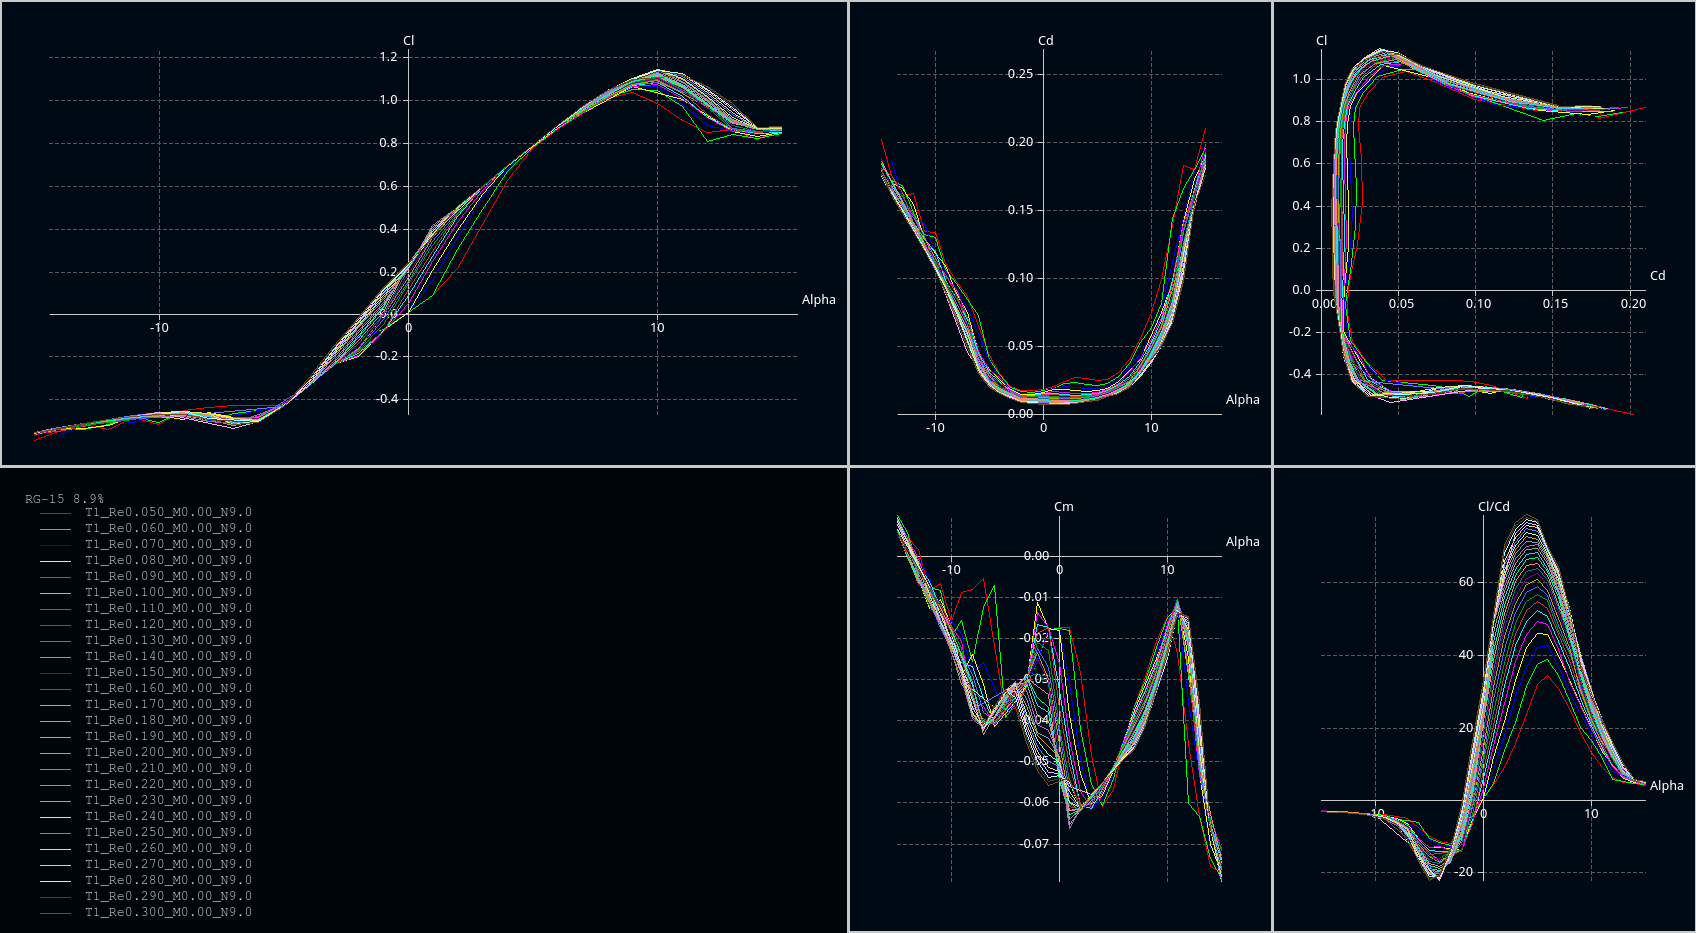
\includegraphics[scale=0.4]{rg15_batch}
\caption{RG15 Airfoil Batch Analysis}
\end{figure}

\begin{figure}[H]
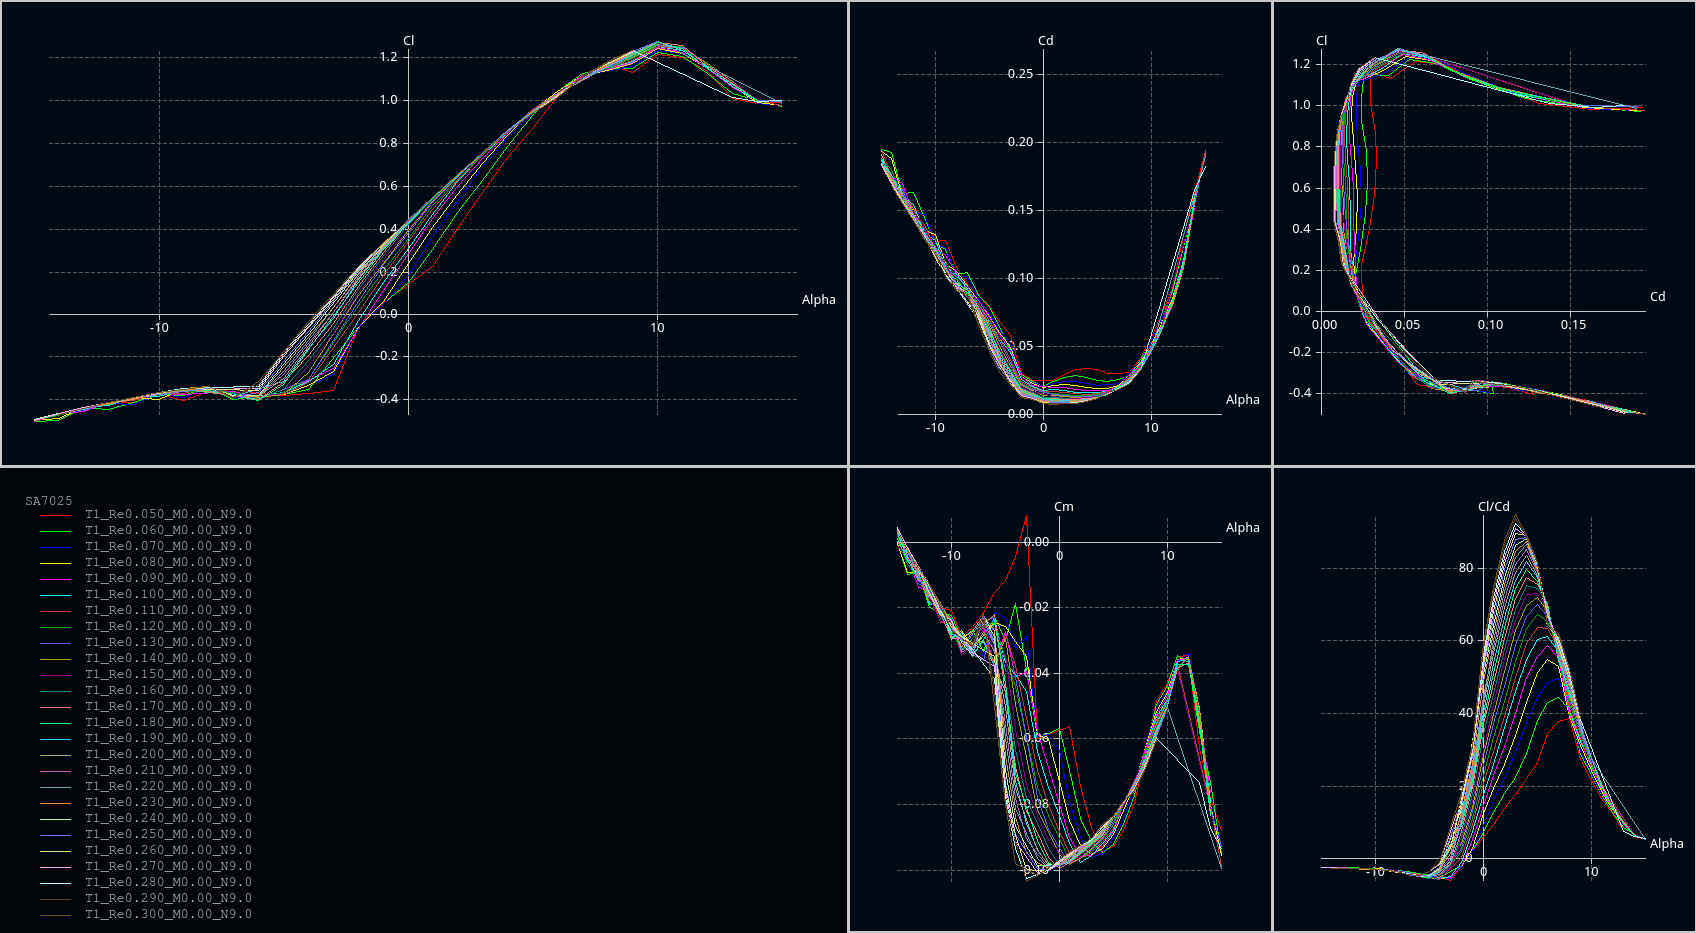
\includegraphics[scale=0.4]{sa7025_batch}
\caption{SA7025 Airfoil Batch Analysis}
\end{figure}

\begin{figure}[H]
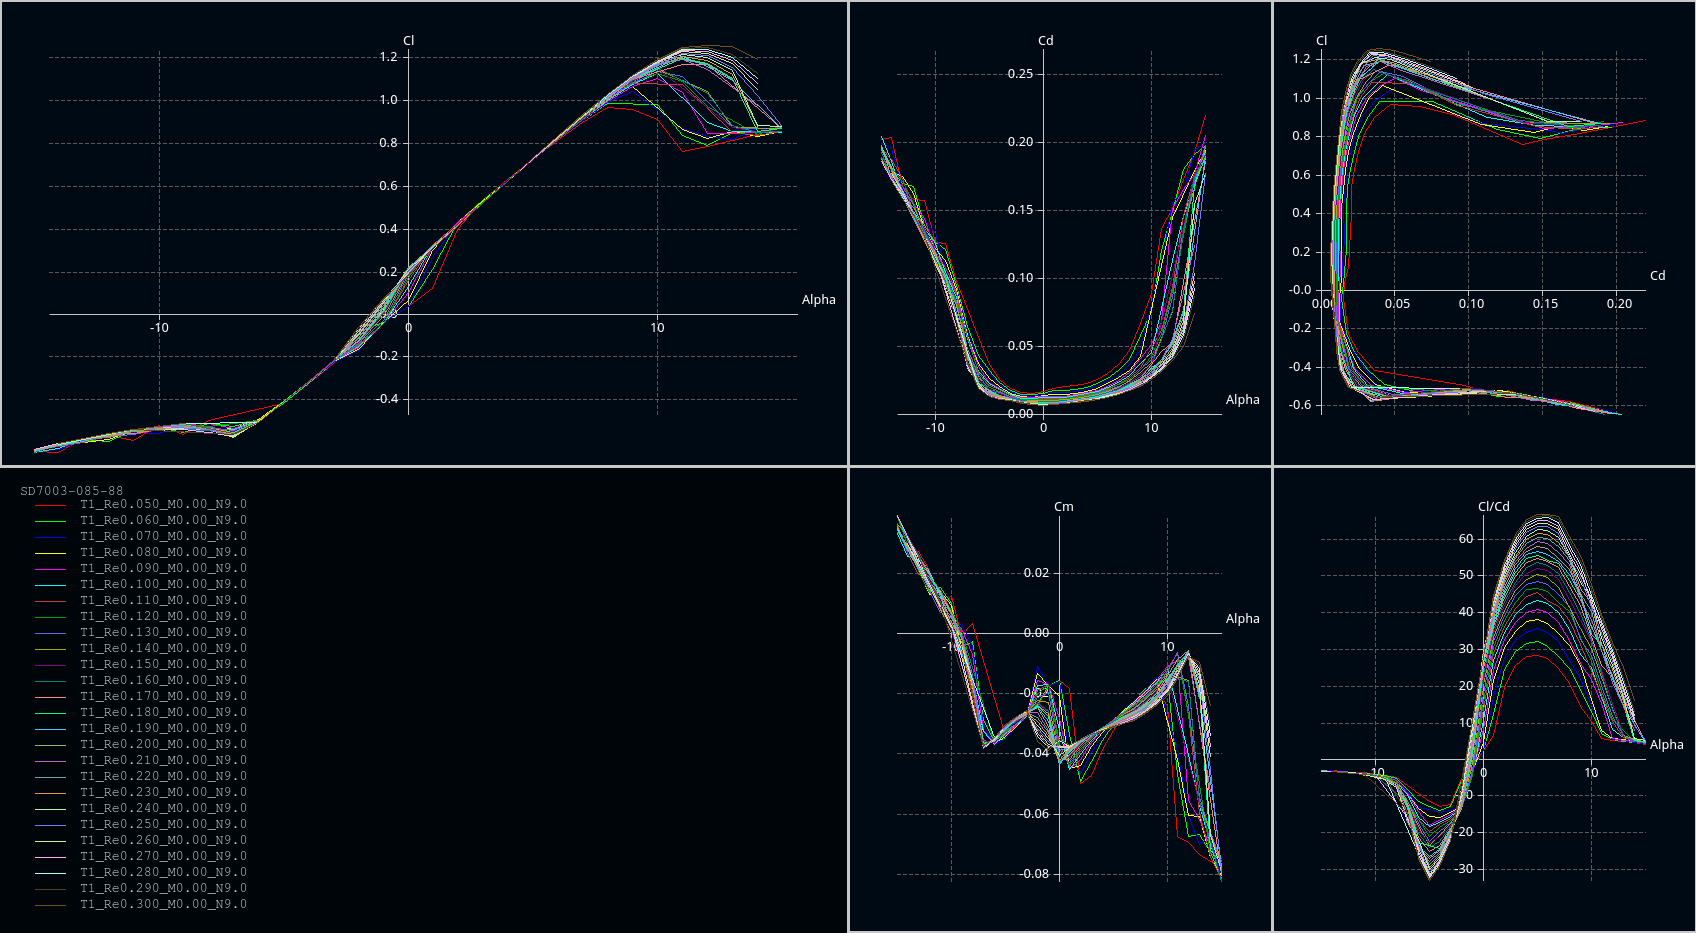
\includegraphics[scale=0.4]{sd7003085_batch}
\caption{SD7003085 Airfoil Batch Analysis}
\end{figure}

\section{3D Finite Wing Analysis}
This section will contain aerodynamic textbook references regarding 3-dimensional flow, it will also contain information about flight stability from a flight mechanics text book. Lastly it will contain visuals of all 3D analysis done 

\section{Wing Loading/Structural Analysis}
May be combined w/ above section
\section{Fuselage Design}

\section{Tail Design}

\section{Propulsion System}
The propulsion system must be lightweight and efficient. The aircraft will be propeller driven, requiring a battery-powered motor. There are three options for motor selection: brushed, inner brushless, and outrunner brushless.
A brushed electric motor is an internally commutated electric motor. A commutator requires electrical contacts called brushes to make contact with it as it rotates. These brushes require periodic maintenance or replacement as they wear out. 
Brushless motors can be categorized as inrunner brushless or outrunner brushless. Brushless motors are electronically commutated, which means they use an electronic controller instead of a brush. The electronic controller does not wear out like a brush, however it can cause an increase in price. The inrunner brushless motor is considered the standard brushless motor, which contains the rotational core within the motor. Inrunner motors can typically supply a high rotational speed with low torque, and should be used with a gearbox. The outrunner brushless motor spins its outer shell around its core, reducing moving parts. The outrunner spins at a lower rotational speed than the inrunner and delivers a higher torque, eliminating the need for a gearbox and reducing weight. However, because the outer surface of the motor rotates, there is no direct way to attach a heat sink and may cause high temperatures in the aircraft. 
The reliability of a brushless motor makes it the best choice. The outrunner brushless motor contributes to a more simple and lightweight design due to the elimination of a gearbox. According to “Aerodynamic and Structural Design of a Small Nonplanar Wing UAV,” the elimination of a gearbox provides a weight savings of 13.3 percent. Many COTS outrunner brushless motors are being specifically manufactured for UAS use, increasing their popularity and reducing their price. The outrunner brushless motor is the preferred choice for the propulsion system, with the consideration that it may need a dedicated cooling system.

\section{Materials}
Discuss available materials through 3D printing facility

\section{Batteries}



\bibliographystyle{plain}
\bibliography{UAS}

\end{document}
